\documentclass{article}
\usepackage[utf8x]{inputenc}
\usepackage{ucs}
\usepackage{amsmath} 
\usepackage{amsfonts}
\usepackage{marvosym}
\usepackage{wasysym}
\usepackage{upgreek}
\usepackage[english,russian]{babel}
\usepackage{graphicx}
\usepackage{float}
\usepackage{textcomp}
\usepackage{hyperref}
\usepackage{geometry}
  \geometry{left=2cm}
  \geometry{right=1.5cm}
  \geometry{top=1cm}
  \geometry{bottom=2cm}
\usepackage{tikz}
\usepackage{ccaption}
\usepackage{multicol}

\usepackage{listings}
%\setlength{\columnsep}{1.5cm}
%\setlength{\columnseprule}{0.2pt}

\usepackage{colortbl,graphicx,tikz}
\definecolor{X}{rgb}{.5,.5,.5}

\title{ДЗ. Работа с изображениями в формате \texttt{.ppm}}
\date{}
\begin{document}
\pagenumbering{gobble}

\lstset{
  language=C,                % choose the language of the code
  basicstyle=\linespread{1.1}\ttfamily,
  columns=fixed,
  fontadjust=true,
  basewidth=0.5em,
  keywordstyle=\color{blue}\bfseries,
  commentstyle=\color{gray},
  stringstyle=\ttfamily\color{orange!50!black},
  showstringspaces=false,
  %numbers=false,                   % where to put the line-numbers
  numbersep=5pt,
  numberstyle=\tiny\color{black},
  numberfirstline=true,
  stepnumber=1,                   % the step between two line-numbers.        
  numbersep=10pt,                  % how far the line-numbers are from the code
  backgroundcolor=\color{white},  % choose the background color. You must add \usepackage{color}
  showstringspaces=false,         % underline spaces within strings
  captionpos=b,                   % sets the caption-position to bottom
  breaklines=true,                % sets automatic line breaking
  breakatwhitespace=true,         % sets if automatic breaks should only happen at whitespace
  xleftmargin=.2in,
  extendedchars=\true,
  keepspaces = true,
}
\lstset{literate=%
   *{0}{{{\color{red!20!violet}0}}}1
    {1}{{{\color{red!20!violet}1}}}1
    {2}{{{\color{red!20!violet}2}}}1
    {3}{{{\color{red!20!violet}3}}}1
    {4}{{{\color{red!20!violet}4}}}1
    {5}{{{\color{red!20!violet}5}}}1
    {6}{{{\color{red!20!violet}6}}}1
    {7}{{{\color{red!20!violet}7}}}1
    {8}{{{\color{red!20!violet}8}}}1
    {9}{{{\color{red!20!violet}9}}}1
}

\title{Семинар \#10: Файлы. Работа с изображениями. Домашнее задание.\vspace{-5ex}}\date{}\maketitle

\begin{center}
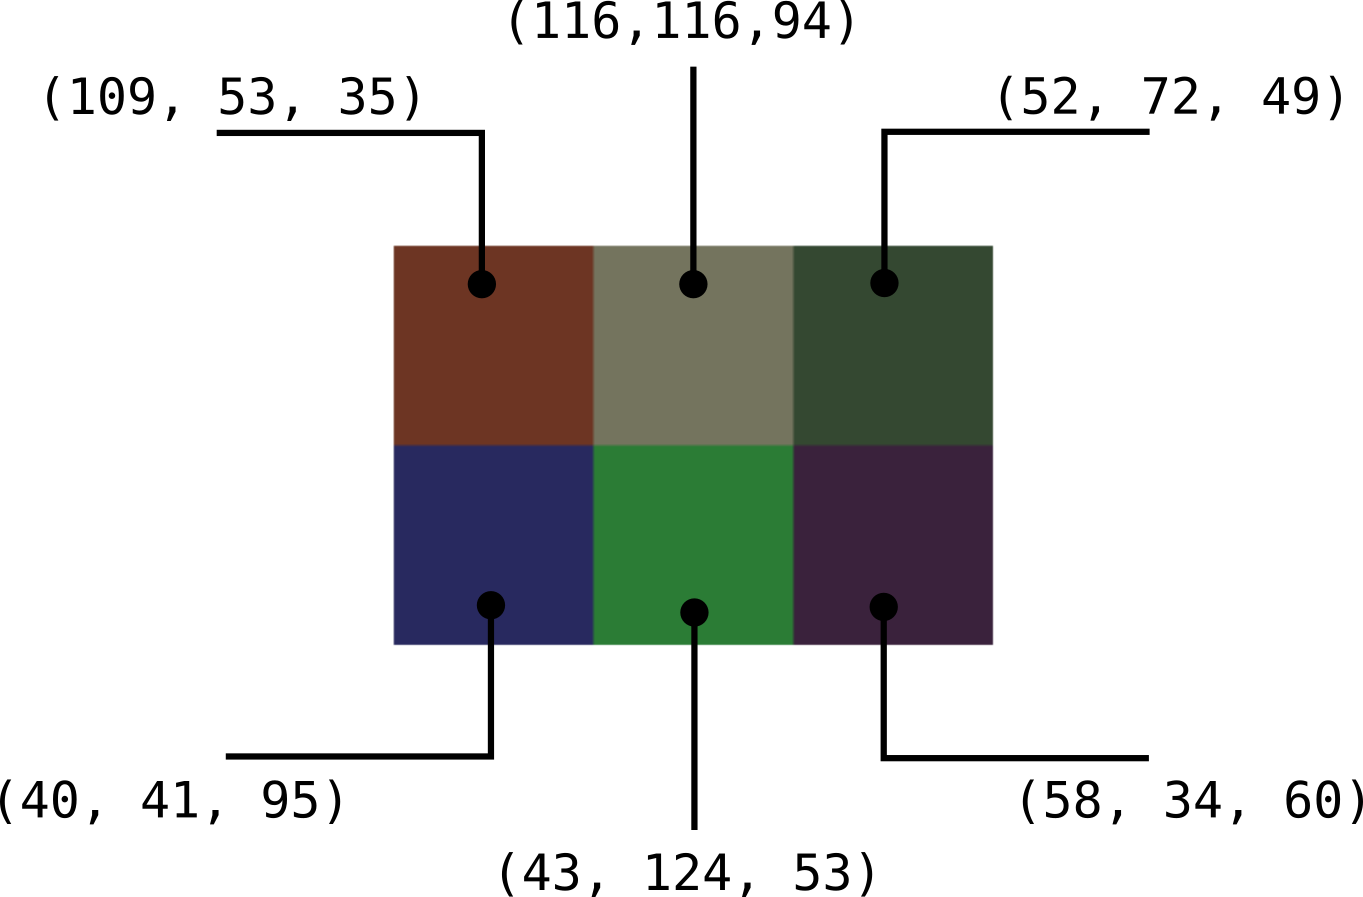
\includegraphics[scale=0.65]{../images/tiny_new_wn.png}
\end{center}

\href{https://ru.wikipedia.org/wiki/Portable_anymap}{\texttt{ppm}} - это простейший формат для хранения изображений. В отличии от других, более продвинутых форматов (например \texttt{jpg} или \texttt{png}), он не использует никаких хитрых алгоритмов сжатия, а просто хранит RGB значения каждого пикселя. Представленное выше крохотное изображение (3 на 2 пикселя) может быть представлено в формате \texttt{ppm} двумя эквивалентными способами - текстовом и бинарном. Цвета картинки специально подобраны так, чтобы в бинарном представлении получались печатаемые символы из таблицы ASCII (символы с кодами от 32 до 126). Так бывает не всегда. Если значение компоненты цвета выйдет за эти пределы, то текстовый редактор напечатает какой-нибудь непонятный символ(какой именно -- зависит от кодировки) или вообще ничего не напечатает. Вот как будет выглядеть \texttt{ppm}-изображение выше, если открыть его в текстовом редакторе:\\


\begin{multicols}{2}
\textbf{Текстовый формат}\\
\begin{verbatim}
P3
3 2
255
109 53 35 116 116 94 52 72 49 
40 41 95 43 124 53 58 34 60
\end{verbatim}
\vfill\null
\columnbreak
\textbf{Бинарный формат}\\
\begin{verbatim}
P6
3 2
255
m5#tt^4H1()_+|5:"<
\end{verbatim}
\vfill\null
\end{multicols}

Побайтовое представление файлов:
\begin{multicols}{2}
\begin{verbatim}
50 33 0a 33 20 32 0a 32 35 35 0a 31 30
39 20 35 33 20 33 35 20 0a 31 31 36 20 
31 31 36 20 39 34 20 0a 35 32 20 37 32 
20 34 39 0a 34 30 20 34 31 20 39 35 20 
0a 34 33 20 31 32 34 20 35 33 20 0a 35 
38 20 33 34 20 36 30
\end{verbatim}
\vfill\null
\columnbreak
\begin{verbatim}
50 36 0a 33 20 32 0a 32 35 35 0a 6d 35
23 74 74 5e 34 48 31 28 29 5f 2b 7c 35 
3a 22 3c
\end{verbatim}
\end{multicols}


Для справки - коды ASCII нужных символов:\\
\begin{tabular}{ccc | ccc} 
\rowcolor[rgb]{0,0.173,0.3255}
\textcolor{white}{Символ}\quad&\textcolor{white}{ASCII-код}\quad&\textcolor{white}{ASCII-код в 16-ричной системе}&
\textcolor{white}{Символ}\quad&\textcolor{white}{ASCII-код}\quad&\textcolor{white}{ASCII-код в 16-ричной системе}
\\ 
\rowcolor[rgb]{0.89451,0.93588,0.97078} 
P                & 80 & 50       &         0  & 48 & 30 \\
пробел           & 32 & 20       &         1  & 49 & 31  \\
\textbackslash n & 10 & 0a       &         2  & 50 & 32  \\
m                & 109& 6d       &         3  & 51 & 33  \\
\#               & 35 & 23       &         4  & 52 & 34  \\
t                & 116 & 74      &         5  & 53 & 35 
\end{tabular}\\
\\
В файле \texttt{tiny.c} представлена программа, в которой создаются 2 файла изображения. Скомпилируйте эту программу и запустите. Создадутся 2 файла: изображение данной маленькой картинки в текстовом и бинарном форматах.

\newpage

В этих задачах вам понадобится программа для просмотра изображений в формате \texttt{ppm}. Если у вас нет программы, которая поддерживает этот  формат на компьютере, то советую использовать IrfanView: \href{https://www.irfanview.com/}{www.irfanview.com}.
В этой программе по умолчанию используется сглаживание при приближении. Его можно отключить, чтобы было видно каждый пиксель \texttt{View -> Display Options -> Use Resample for zooming} (убрать галочку).
\subsection*{Рисование в файл изображения}

\begin{itemize}
\item \textbf{Флаг:} В файле \texttt{flag.c} содержится пример работы создания изображения в формате \texttt{.ppm} в программе. Напишите программу, которая будет рисовать флаг Японии. Изображение должно иметь размер 600 на 400 пикселей. Компоненты белого цвета: \texttt{(255, 255, 255)}. Компоненты красного цвета: \texttt{(190, 0, 41)}.
\begin{center}
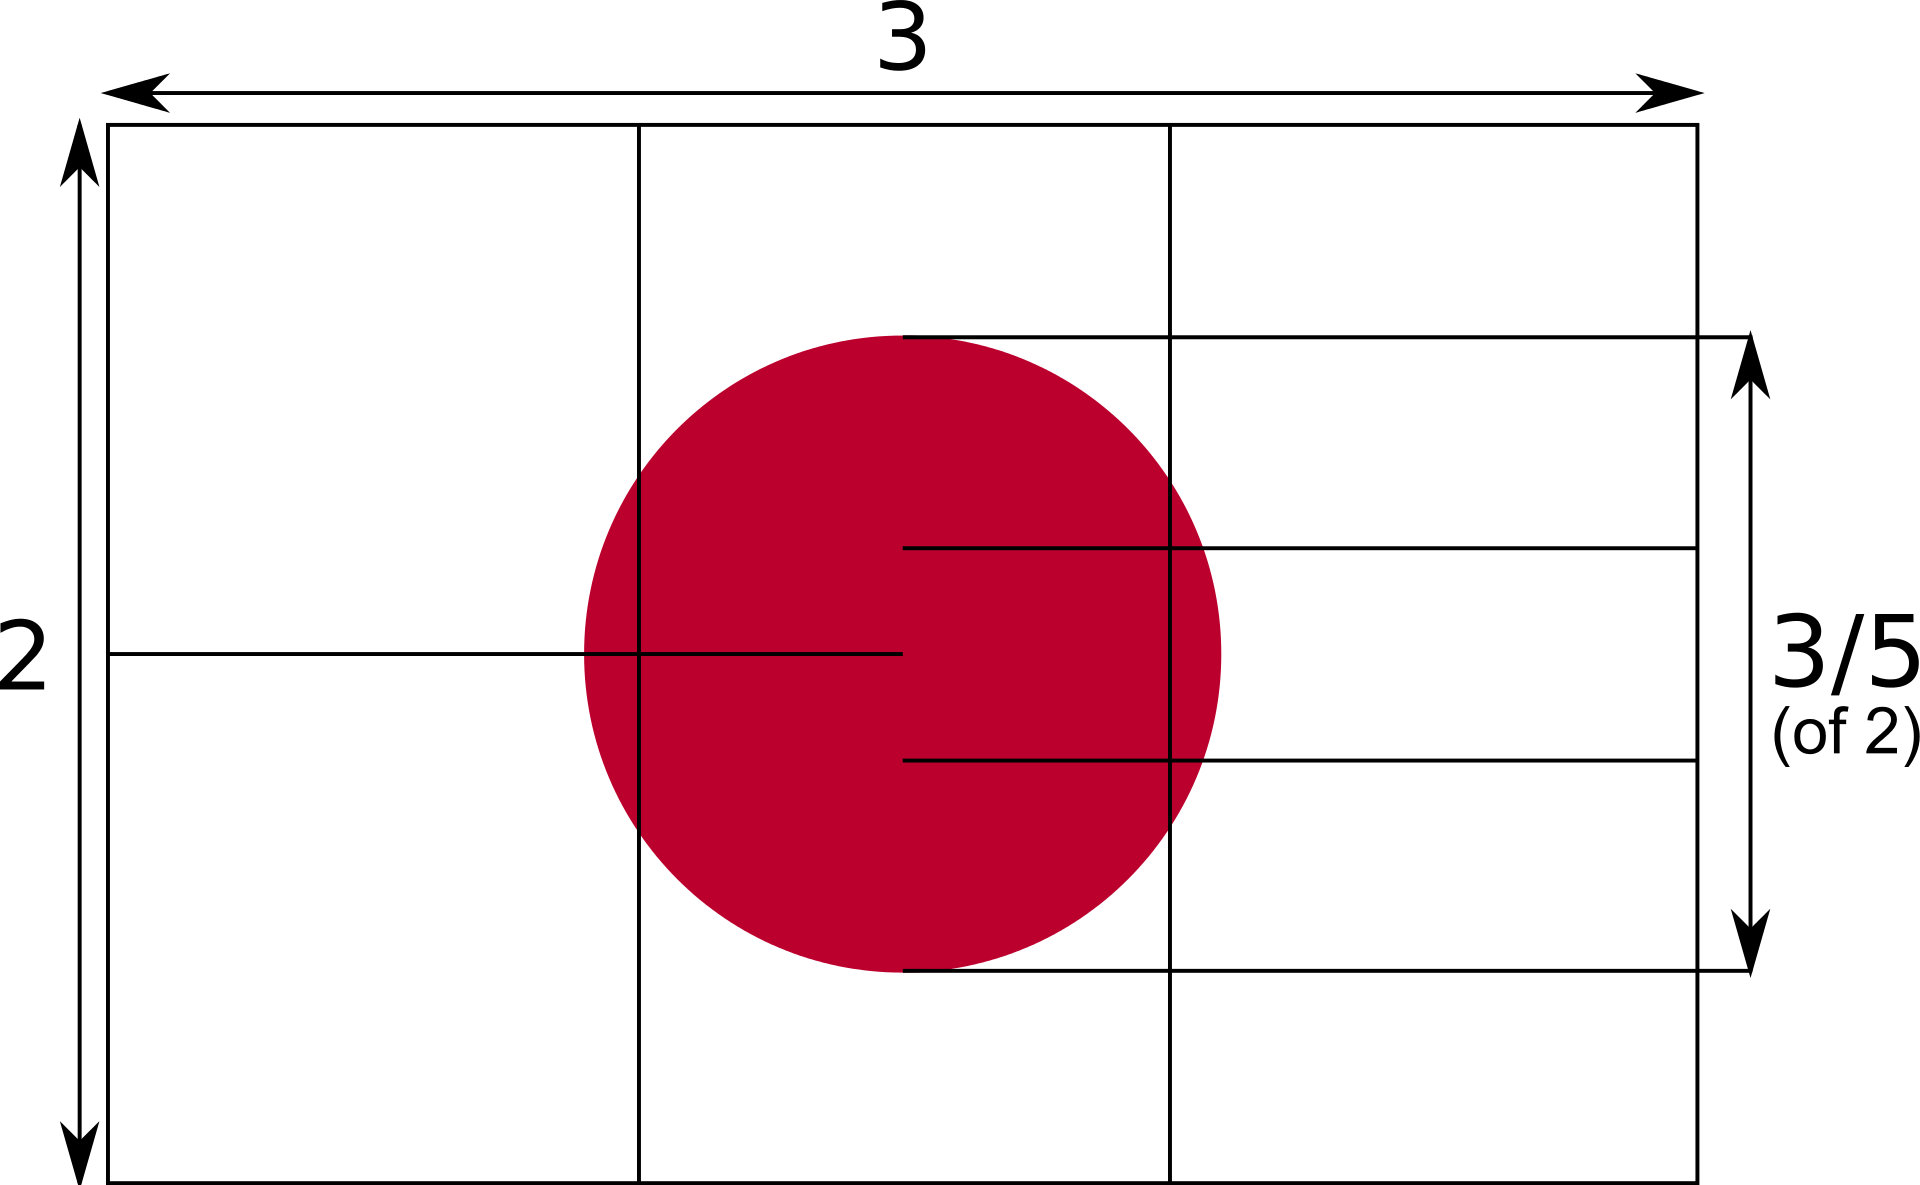
\includegraphics[scale=0.15]{../images/japanflag.png}
\end{center}
\item \textbf{Случайные круги:} 
\begin{itemize}
\item Напишите функцию \\
\texttt{void draw\_circle(Color* data, int width, int height, int x0, int y0, int r, Color c)}\\
которая будет рисовать круг на холсте \texttt{data} с центром в точке \texttt{(x0, y0)}, радиусом \texttt{r} и цветом \texttt{c}.
\item Напишите программу, которая будет рисовать \texttt{n} кругов случайного цвета, расположения. Радиус тоже выбирается случайный в диапазоне от \texttt{a} до \texttt{b}. Параметры \texttt{n}, \texttt{a} и \texttt{b} передаются через аргументы командной строки. Программа должна создавать изображение \texttt{circles.ppm}.
\end{itemize}
\item \textbf{Функция двух переменных:} Напишите программу, которая будет рисовать значения функции двух переменных $f(x, y)$ в области $[-1, 1]\times[-1, 1]$.\\
 Значения функции должны сохранятся в изображении размером 500 на 500 пикселей. К примеру, пиксель с координатами \texttt{(250, 250)} должен хранить значение функции в точке $(0, 0)$, а пиксель \texttt{(0, 400)} - значение в точке $(-1, 0.6)$. \\
Учтите, что значения пикселей изображения должны лежать в интервале от 0 до 255. Постройте изображения следующих функций: 
\begin{enumerate}
\item $f(x, y) = k\cdot|x \cdot y|$
\item $f(x, y) = k\cdot|sin(10\cdot(x^2 + y^2))|$
\item $f(x, y) = k\cdot|sin(5000\cdot(x^2 + y^2))|$
\item $f(x, y) = k\cdot|cos(10x)\cdot sin(10y)|$
\item $f(x, y) = k\frac{1}{2}\cdot\Big|sin\Big(\frac{3}{0.1 + |x|}\Big) + sin\Big(\frac{3}{0.1 + |y|}\Big)\Big|$
\end{enumerate}
Параметр $k = 255$ подбирается так, чтобы значения компонент цвета лежало в диапазоне от 0 до 255.
\end{itemize}
\newpage
\subsection*{Обработка изображений}
В файле \texttt{brightness.c} содержится программа, которая увеличивает яркость изображения. Используйте её как пример для решения следующих задач. Компиляция и запуск этой программы осуществляется следующим образом:
\begin{verbatim}
gcc -std=c99 -o brighter brightness.c
./brighter images/emir.ppm 50
\end{verbatim}
\begin{itemize}
\item \textbf{Черно-белое изображение:} Написать программу, которая принимает на вход файл изображения, считывает его и превращает в чёрно-белое изображение и записывает в файл \texttt{result.ppm}. Название изображения должно передаваться через аргументы командной строки.
\item \textbf{Перестановка цветов:} Написать программу, которая переставляет местами красную и синюю компоненты цвета. Применить её на файле \texttt{emir.ppm}.
\item \textbf{Сепия:} Написать программу, которая будет применять к изображению эффект сепии.
\begin{multicols}{3}
Формулы для эффекта сепии:
\begin{align*}
r_{new} = 0.393 \cdot r + 0.769 \cdot g + 0.189 \cdot b\\
g_{new} = 0.349 \cdot r + 0.686 \cdot g + 0.168 \cdot b\\
b_{new} = 0.272 \cdot r + 0.534 \cdot g + 0.131 \cdot b\\
\end{align*}
Если какое-то из этих значение станет большим, чем $255$, то его нужно приравнять к $255$.
\vfill			
\begin{center}
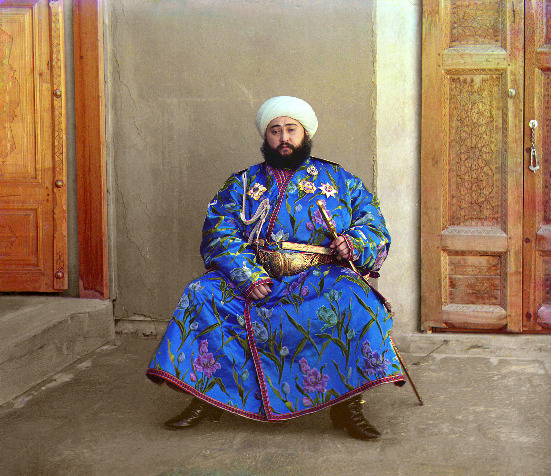
\includegraphics[scale=0.26]{../images/imageproc.jpg}
\end{center}
\vfill			
\begin{center}
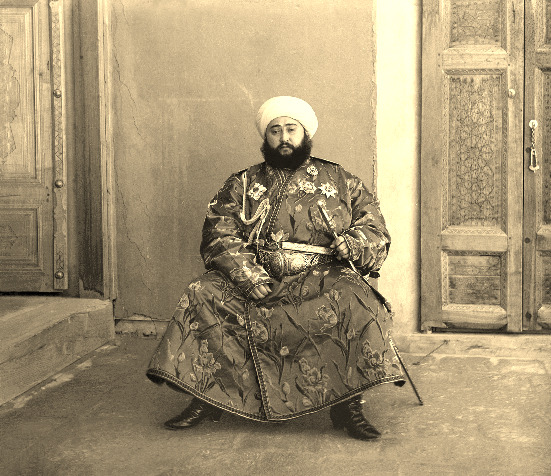
\includegraphics[scale=0.26]{../images/imageproc_sepia.jpg}
\end{center}
\end{multicols}
\item \textbf{Отражение:} Напишите программу, которая зеркально отражает изображение по вертикали (относительно горизонтальной прямой).
\item \textbf{Свёртка изображения. Размытие.}
Операция свёртки изображения задаётся следующей формулой:
\begin{align*}
data_{new}[i, j] = \sum_{p=-1}^{1} \sum_{q=-1}^{1} K[p+1, q+1] \cdot data[i+p, j+q]\\
\end{align*}
, где $K$ - некоторая матрица 3 на 3. Для размытия эта матрица равна:
$$
K = 
\frac{1}{9}
\begin{pmatrix}
1 & 1 & 1 \\
1 & 1 & 1 \\
1 & 1 & 1
\end{pmatrix}
$$\\

Подробней о свёртке можно посмотреть тут:
 \href{https://www.youtube.com/watch?v=C_zFhWdM4ic&t=74s}{\texttt{www.youtube.com/watch?v=C\_zFhWdM4ic}}\\
Если провести эту операцию 1 раз, то размытие будет небольшое. Чтобы размыть изображение сильнее нужно повторить эту операцию несколько раз.
Напишите программу, которая будет размывать изображение \texttt{n} раз (\texttt{n} передаётся через аргументы командной строки).


\iffalse
\item \textbf{Нахождение границ:} Для нахождения вертикальных или горизонтальных границ на изображении, сначала нужно превратить это изображение в черно-белое, а затем применить свёртку со следующей матрицей:
\begin{multicols}{2}
$$
K_1 = 
\frac{1}{k}
\begin{pmatrix}
-1 & 0 & 1 \\
-2 & 0 & 2 \\
-1 & 0 & 1
\end{pmatrix}
$$\\
\vfill
$$
K_2 = 
\frac{1}{k}
\begin{pmatrix}
1 & 2 & 1 \\
0 & 0 & 0 \\
-1 & -2 & -1
\end{pmatrix}
$$\\
\end{multicols}
Параметр $k$ настраивается. Обычно $k \approx 50$.\\
Изображение, содержащее все границы находится применением оператора $K = \sqrt{K_1^2 + K_2^2}$.
\fi
\item \textbf{Консольный графический редактор:} Объедините все решения предыдущих задач в одну программу \texttt{mge}. Выбор эффекта должен задаваться с помощью аргументов командной строки. Например так:
\begin{verbatim}
mge --sepia image.ppm result.ppm
\end{verbatim}
Программа должна применять эффект сепии на изображение \texttt{image.ppm} и сохранять результат в \texttt{result.ppm}.

А при таком вызове программа должна применять эффект размытия 10 раз:
\begin{verbatim}
mge --blur 10 image.ppm result.ppm
\end{verbatim}
Добавьте ещё опции: \texttt{----brighter}, \texttt{----bw}, \texttt{----changecolors}, \texttt{----mirror}.
\end{itemize}

\newpage
\subsection*{Рисование линий. Алгоритм Брезенхема:}

Алгоритм построения прямой линии между двумя точками на двумерном холсте называется алгоритмом Брезенхема.
В файле \texttt{4lines.c} есть реализация этого алгоритма на языке \texttt{C}.
\begin{center}
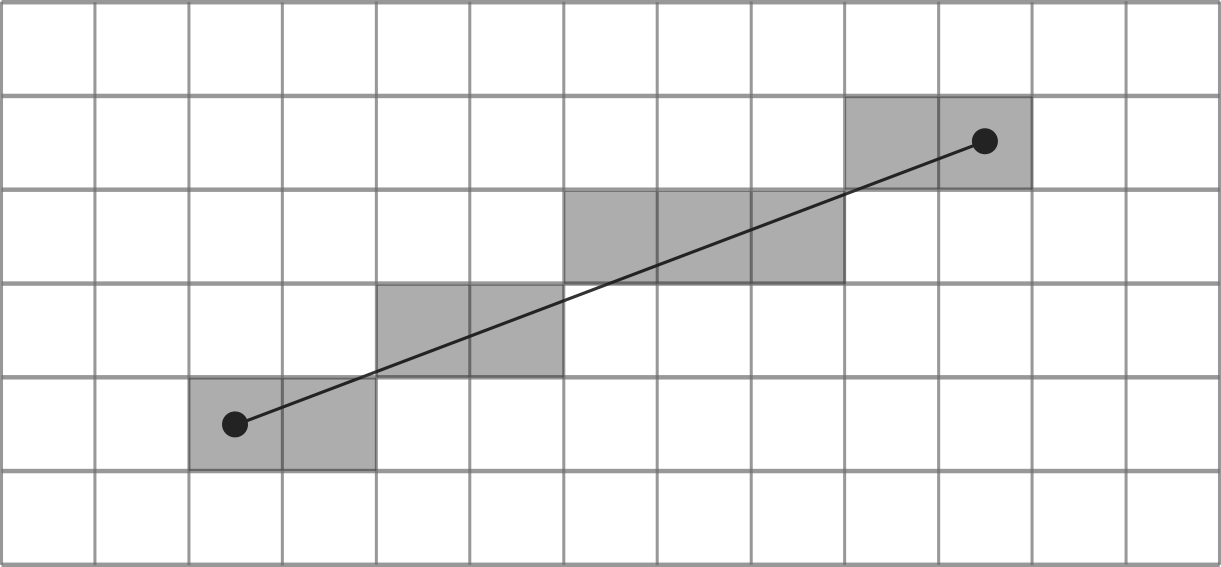
\includegraphics[scale=1]{../images/bresenham.png}
\end{center}

\begin{itemize}
\item \textbf{Случайные линии:}\\
Создать программу, которая будет рисовать \texttt{n} случайных отрезков случайного цвета. \texttt{n} должен передаваться через аргументы командной строки. Программа должна создавать файл \texttt{randlines.ppm}.
\item \textbf{Фрактальное дерево:}\\
Напишите рекурсивную функцию, которая будет рисовать фрактальное дерево:
\begin{center}
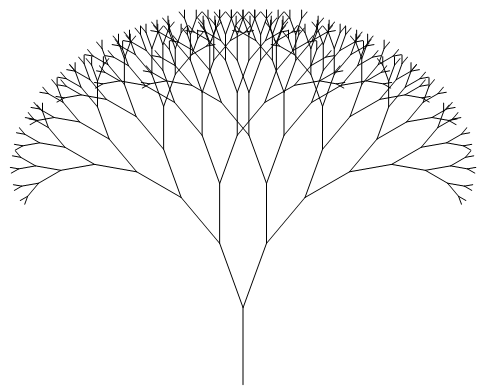
\includegraphics[scale=0.4]{../images/treefractal.png}
\end{center}
\end{itemize}

\subsection*{Работа с изображениями формата \texttt{.jpg} и \texttt{.png}:}
Популярные форматы изображений такие как \texttt{.jpg} или \texttt{.png} имеют сложную структуру, так как используют хитрые алгоритмы сжатия. Про \texttt{jpg} можно посмотреть тут:\\
 --> \href{https://www.youtube.com/watch?v=8N0Bx8DMt6c}{www.youtube.com/watch?v=8N0Bx8DMt6c}\\
Считывать файлы таких форматов самостоятельно было бы очень непросто, так как нужно было бы досконально знать строение файла изображения. К счастью делать это необязательно, так как уже всё сделано за нас другими программистами. Есть простая библиотека \texttt{stb\_image}. Эта библиотека подключается простым \texttt{include} (что не справедливо для большинства других библиотек). Пример работы с библиотекой -- в папке \texttt{stb}.
\begin{itemize}
\item \textbf{jpeg редактор:} Измените программу из задачи консольный графический редактор так, чтобы она работала с форматом \texttt{.jpg}. Добавьте параметр командной строки \texttt{quality}, который будет задавать качество получаемой \texttt{jpg}-картинки. 
\end{itemize}

\end{document}